\chapter{Conclusion}
\label{chap:conclusion}
\section{Summary}
The goal of this project was to create a system to help to build an intuitive understanding of functional programming languages work. I identified two groups of stakeholders for this goal:

\begin{itemize}
    \item Those involved in teaching functional languages, as part of a university course or otherwise. They could such a tool to demonstrates functional languages to facilitate intuitive explanations in lectures.
    \item Those involved in learning functional languages. These could be students of a university course, or anyone interested in the topic. They could use such a tool to experiment with functional languages. 
\end{itemize}

\noindent I created SFL Explorer, which includes a functional programming language \ac{SFL} with a simple but effective set of features, and a UI that allows users to interact with the evaluation of the program in real time, building intuition for how functional languages work. I tested this project with 27 different students and 2 lecturers in functional programming to represent my two groups of stakeholders. This was done throughout the project to ensure that the development of SFL Explorer  evolved in a way that met the goals for each group of stakeholders. 

Below is a summary of the four phases of the project, and what was achieved in each. 
\paragraph{Phase 1 --- Proof of Concept} I performed requirements analysis based on discussions with my supervisor and using autoethnographic methods. These requirements came together to create the idea for SFL Explorer, and then went on to inform the design of the language \ac{SFL} and the Explorer (the website). The language was very minimal, based on \lcalc~with only a few minor additions. This was then implemented, along with a proof of concept iteration of the website. The proof of concept was presented to my client, Samantha Frohlich, a lecturer on~\hyperref[COMS10016]{COMS10016}, who was positive about the project, and gave good feedback about future iterations of the system, particularly on the language. 
\paragraph{Phase 2 --- Types and Pattern Matching} This phase was mostly about extending the language, adding the features requested by my client. This included a type system, polymorphism, user definable algebraic data types, recursive data types, and pattern matching. I also successfully implemented a typechecker that supports the \ac{SFL} type system based on Dunfield and Krishnaswami's bidirectional type checking algorithm~\cite{completebidir}. I then held a focus group with functional programming experts where we discussed the language, and what could be done to make the UI/UX better. 
\paragraph{Phase 3 --- Improving the UI/UX} In this phase, I overhauled the UI/UX, and added features to make it easier to use, including syntax highlighting, difference between steps, and reductions messages. I held a focus group with some students who had just been through a university functional programming course, but found it difficult. In this focus group, students were taught functional programming using SFL Explorer  in a lecturer setting, and then interviewed about what they found useful/not so useful about SFL Explorer . These students really liked the system, but there were also definitely things that could be improved, some of which were worked on in the final phase, and some are listed as future work. 

\paragraph{Phase 4 --- Further UI/UX Iteration} This phase was mostly tweaks to the UI as suggested by previous focus groups, including syntax highlighting, and fixes to visual bugs. I also added untyped mode, and the ability to disable the prelude. This then concluded with the final focus group which followed the same split lecture/interview format as the last focus group, followed by a meeting with my client. 


\section{Strengths}
\subsection{The System is Useful for Teaching Functional Programming, and Will be Used for that Purpose}
All three focus groups found the system useful. In particular, the intermediate focus group who had just taken the Haskell unit, all agreed that they would have benefitted from this system in the module. 
As discussed previously \ref{c4:client}, my client will use this project in future in teaching \hyperref[COMS10016]{COMS10016}. Furthermore, she shared it with a teaching fellow who teaches Haskell at Imperial, who agreed that it is useful. 

\subsection{The Language Achieves Its Design Aims}
See \ref{design:goals} for the initial discussion of the design goals. 

\paragraph{Design Aim 1: `It Should be Simple and Easy to Understand'}
All three focus groups have supported the conclusion that the language is easy to understand. The advanced and intermediate focus groups appreciated the relatively small deviations from Haskell such as the explicit match expressions, and the small set of inbuilts. Indeed, one participant in the intermediate focus group said that they thought the explicit matching syntax was much easier to understand than Haskell's pattern matching, saying it was better for learning \ref{eval:IFG}. The beginner focus group also had little difficulty grasping the syntax and semantics of the language in a lecture context, however they would have found it harder without guidance. Sentiment was more divided about the fact that \sflinline{Cons} is not an infix operator


\paragraph{Design Aim 2: `It Should be Similar to Existing Functional Languages'}
Both the advanced and intermediate focus groups, both with participants that had been formally taught Haskell, had very little trouble understanding the language. 

\paragraph{Design Aim 3: `It Should be Powerful Enough to Explain Key \ac{FP} Concepts'}
Amos Holland used SFL Explorer  to explain key concepts to the intermediate \ref{eval:IFG} and beginner \ref{eval:BFG} focus groups. 

\begin{quotation}
\noindent `There are features of Haskell it doesn't have, but Haskell is a very advanced language. For teaching functional programming, I think it's got the right range of features'. Amos Holland, During an interview after lecturing in the intermediate focus group.
\end{quotation}

\noindent The language is also capable of doing everything that my client mentioned that she wanted to use such a system for (\ref{eval:c1_client}).


\section{Limitations}
Here, I have only listed a few `limitations'. This is not to say that there is nothing else that could be added to the project, far from it (see~\ref{conc:future_work}). These are the only things that I have identified as problems with the existing system as opposed to extensions that could be made to it. 

\subsection{Related Redexes are Confusing in Free Choice Mode}
In free choice mode some redexes may include other redexes. Consider the following \ac{SFL} program:

\begin{lstlisting}[language=SFL]
main :: a -> Int 
main = (\x y z. x + y) 1 2
\end{lstlisting}

\noindent If we evaluate this in free choice mode, we are presented with two options:
% \begin{alignat}{3}
% \verb|(\x. \y. \z. x + y) 1 2| & $\smallblacktriangle*$ &  \verb|\z. 1 + 2| \\ 
% \end{alignat}

\begin{figure}[!h]
    \centering
    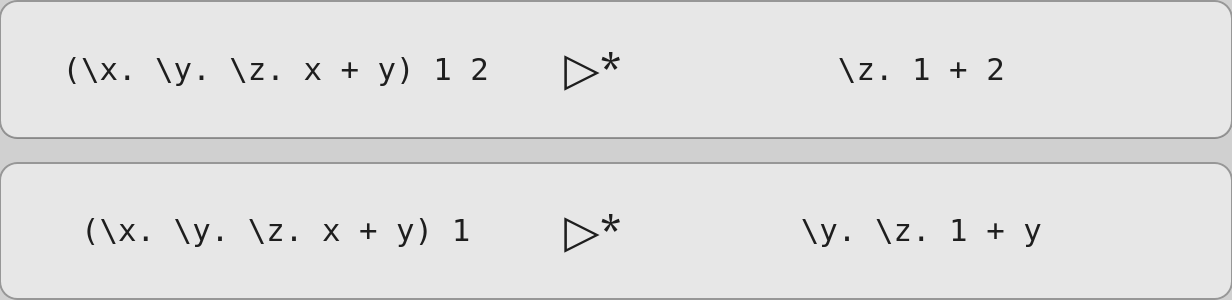
\includegraphics[width=0.75\linewidth]{images/conc_add_3.png}
\end{figure}

\noindent The first option is two reductions, the first of which is the second one. This relationship is not clear. This was discussed in the advanced focus group~\ref{ref:afg}, but development of a fix for this was not prioritized. 

\subsection{The Expressions Balloon During Evaluation}
\label{conc:baboon}
I believe that the languages lack of inbuilts is one of the languages best `features'. However, it is also a curse. Because everything is defined with match expressions, the expression balloons vertically with match statements during evaluation. For instance, in the provided `square\_sum' example:

% \begin{figure}[h]
\begin{lstlisting}[language=SFL]
square :: Int -> Int
square x = x * x

// List of the square numbers from lower to upper
list_of_squares :: Int -> Int -> List Int
list_of_squares lower upper = map square $ range lower upper

main :: Int
main = sum $ list_of_squares 1 5
\end{lstlisting}
% \end{figure}

\noindent Despite their being no match expressions, the `main' expression balloons to 3 match statements deep within 6 lazy steps:

% \begin{figure}[h]
\begin{lstlisting}[language=SFL]
match (match (match (infiniteFrom 1) {
    | Nil -> Nil
    | Cons x xs -> if ((5 - 1) > 0) (Cons x (take ((5 - 1) - 1) xs)) Nil
}) {
    | Nil -> Nil
    | Cons x xs -> Cons (square x) (map square xs)
}) {
    | Nil -> 0
    | Cons x xs -> (\x. \acc. x + acc) x (foldr (\x. \acc. x + acc) 0 xs)
}
\end{lstlisting}
% \end{figure}

\noindent The outer one comes from `sum', the middle one comes from `map', and the inner one comes from `range', all prelude functions. Unfortunately, this is hard to avoid, as pattern matching is a key concept in functional programming languages. Furthermore, a conclusion of the intermediate focus group was that the explicit match syntax, where it was obvious where/how pattern matching was occurring, made understanding pattern matching much easier. Indeed, they agreed that they would have liked to have SFL to learn about pattern matching rather than Haskell (see \ref{eval:IFG}). 

This situation could be improved by being able to select which functions we are interested in seeing the expansion of, and which ones we are not. See \ref{fw:function_checkboxes}

% \subsection{There is No Documentation}
% When designing the new UI (\ref{c2:next_ui}), I included buttons that would create help menus, and more information about the project, as well as instructions. However, these are time-consuming to write,  and I did not have time. 

\section{Future Work}
\label{conc:future_work}
\paragraph{Add More Documentation to the Website} As the language is quite similar to Haskell, an advanced user would not have much trouble figuring out how the website works. This works fine for a lecture tool as the lecturer would be able to figure it out, but the lack of documentation is detrimental to other users. 
\paragraph{Other Evaluation Strategies}
Users could have the option to pick the evaluation strategy. They can manually pick the evaluation strategy using free choice mode, but a mode that enforces strict evaluation for example would be useful to have. 
\paragraph{Improve Free Choice Mode}
Inspiration could be taken from the UI used by \llessons~\ref{bg:llessons_ui} where the expression to be evaluated could be selected by clicking on the input text itself. 
\paragraph{Keyboard Controls} This was requested by Samantha, my client, in our final meeting~\ref{c4:client}. She requested keyboard controls to be able to step forward and backward using our chosen evaluation strategy. 
\paragraph{Step to the End Button} This feature was requested by Amos during the intermediate focus group~\ref{eval:IFG}. A button would be provided to skip evaluation to the end of the program. This is not as trivial as it sounds, as the program may not terminate, and therefore crash the user's browser in trying to compute the final state. This problem could be avoided if we had keyboard controls, where holding in a certain button would repeatedly evaluate via the chosen reduction strategy. 
\paragraph{Selective Skipping}
\label{fw:function_checkboxes}
We are not always interested in all the functions involved in our program. For instance, if a lecturer is attempting to demonstrate \verb|foldr| over a list, they may not be interested in the expansion of how \verb|range| works in order to generate their list they are going to fold over. They may want the evaluation of some things to be `skipped'. 

We could mark certain expressions as uninteresting, and evaluate them as much as we can immediately. For instance, if the syntax for an uninteresting expression looked like `[e]':

\begin{lstlisting}[language=SFL]
main :: Int 
main = sum $ [range 1 4]
\end{lstlisting}

\noindent We could fully evaluate `\lstinline[language=SFL]|range 1 4|' to `\lstinline[language=SFL]|Cons 1 (Cons 2 (Cons 3 Nil))|'. However, this could cause issues if the term does not evaluate. 

% \begin{lstlisting}[language=SFL]
% fix f = f $ fix f

% id x = x

% main = if true 1 [fix id]
% \end{lstlisting}

% The evaluation of `\lstinline[language=SFL]|fix id|' will never terminate. If we were to attempt to evaluate this, it would run forever. If we were to provide a mechanism that forces full evaluation of a term, we would be providing functionality that the user could use to `shoot themselves in the foot'. This would need to be clearly communicated to the user, and a mechanism of stopping this evaluation should be provided if the user judges it has been too long. 



\paragraph{Extensions to the language}
As suggested by Amos during the intermediate focus group (\ref{eval:IFG}) the language could be extended with typeclasses. 
